\chapter{Especificaciones.}\label{cap:capitulo2}

Definiremos el problema, las especificaciones y directrices tanto del tipo de juego como del sistema de generación. Dichas directrices que delimitarán el sistema a crear, han sido establecidas por la empresa indie de videojuegos \emph{TheGameKitchen}, y el sistema será empleado en un futuro título de la misma.

\section{Género de juego.}

En esta sección abarcaremos el tipo de juego y las directrices establecidas en cuanto al género de juego y otras especificaciones relacionadas con el mundo en el que se desarrollará el mismo.

\subsection{Roguelike}

El género de juego en el que nos basaremos será \emph{roguelike} \cite{rlike}, cuyas características principales son:

\begin{itemize}
	\item \emph{Generación de mazmorras}. Cada vez que el jugador inicia una partida, la experiencia será ligeramente distinta.
	\item \emph{Importancia considerable a la exploración}. El hecho de que las mazmorras no sean siempre iguales, incita al jugador a tener que invertir tiempo en explorar para poder encontrar la salida.
	\item \emph{Desarrollo del juego por plantas}. El objetivo del jugador suele ser llegar a una habitación considerada como final, donde puede elegir entre tomar las escaleras para pasar a una siguiente planta, o investigar un poco más en la presente.
	\item \emph{Dificultad progresiva}. Cada planta, tendrá una dificultad ligeramente mayor a la de la anterior hasta llegar a la última.
	\item \emph{Muerte permanente}. Una vez que el jugador muere, no hay manera de cargar la partida. La unica opción es comenzar de nuevo.
\end{itemize}

Históricamente, el género \emph{roguelike} se identificaba además por otro tipo de características, como la mecánica por turnos o el énfasis en jugabilidad y desinterés en los gráficos, pero con el tiempo, el género se ha ido abriendo paso a una definición más genérica. Debido a ésto, hoy en día existen desde \emph{shooters} considerados \emph{roguelike}, como por ejemplo \emph{Tower of Guns} o \emph{Paranautical Activity}, hasta \emph{plataformas}, como \emph{Risk of Rain} o \emph{Spelunky}.

\subsection{Especificaciones del mundo}

Así, las únicas especificaciones que se han dado en cuanto a las reglas de juego son las siguientes:

\begin{itemize}
	\item Entorno en dos dimensiones
	\item El jugador comenzará en una habitación y tendrá como objetivo llegar a una habitación final
	\item Se empleará una vista cenital (figura~\ref{fig:tileclip}).
\end{itemize}

\begin{figure}[t]
\centering
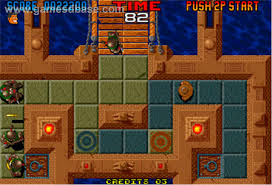
\includegraphics[scale=1]{img/cenital}
\caption{Vista cenital en el juego Action Hollywood por TCH, 1995
\label{fig:cenital}}
\end{figure}

Estas especificaciones son bastante genéricas, por lo que el sistema elaborado podrá servirnos para otro tipo de juegos. Más adelante veremos que se ha procurado dar un enfoque de alta flexibilidad en este aspecto al sistema.

\section{Requisitos del escenario.}

La representación de los escenarios elegida será un mapa de tiles. Como se comentó anteriormente, los mapas de tiles están representados por una matriz, donde cada casilla corresponde a un gráfico de un tamaño normalizado para todos los tiles (un gráfico para las paredes, otro para el suelo, etc). Suelen componerse por capas para añadir decorado, pero para nuestra finalidad, hemos obviado esta característica, ya que se hará hincapié principalmente en la distribución de las habitaciones. No obstante, sería muy sencillo añadir capas como mejora futura.

La optimización en cuanto a clipping (evitar renderizar zonas no visibles) en un mapa de tiles está muy investigada. Debido a que el propio mapa es una rejilla, se puede recorrer y renderizar exclusivamente la zona que va a verse. En la figura~\ref{fig:tileclip} se representa en rojo el viewport del jugador. Los tiles amarillos están en el borde del viewport, y los verdes están completamente dentro. Así, solo hace falta recorrer y dibujar los tiles verdes y amarillos, ahorrándonos el dibujado de los azules.

\begin{figure}[t]
\centering
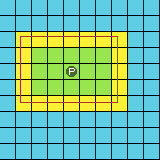
\includegraphics[scale=1]{img/tileclip}
\caption{Clipping en un mapa de tiles
\label{fig:tileclip}}
\end{figure}

Otra característica importante de los mapas de tiles es la sencillez y flexibilidad que da a la hora de componer escenarios; podemos reutilizar tiles y añadir variaciones de los mismos para, en el mapa final, dar sensación de variedad sin tener que elaborar muchos gráficos.

Por todo ello, es un tipo de escenario muy popular desde las antiguas consolas como \emph{NES} o \emph{SNES} hasta hoy.

El escenario estará compuesto por habitaciones, cada una representada como una matriz. Será nuestra tarea plantear un sistema que elabore distribuciones de las habitaciones según los requisitos que se expondrán a continuación.

\section{Directrices para la generación.}

En esta sección explicaremos las directrices impuestas para la generación de los escenarios.


\subsection{Lista inicial de habitaciones}

El sistema que construiremos deberá cumplir una serie de características que analizaremos en detalle en esta sección. Como se ha mencionado previamente, se ha tomado la libertad de añadir características que no estaban en los requisitos previos de \emph{TheGameKitchen}.

El sistema debe generar un mapa de tiles partiendo de una \emph{lista inicial de habitaciones} previamente construida. Para construir las habitaciones, se ha elaborado un editor via web usando el canvas que proporciona HTML y JavaScript (se puede ver en la figura~\ref{fig:roomed}). Así, el objetivo será colocar las habitaciones presentes en esta lista inicial.

\begin{figure}[t]
\centering
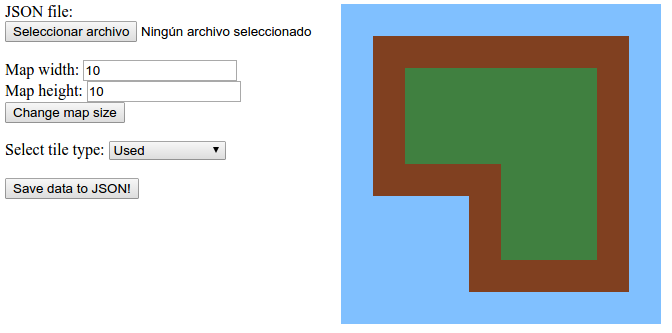
\includegraphics[scale=0.5]{img/roomed}
\caption{Editor de habitaciones
\label{fig:roomed}}
\end{figure}

Las habitaciones \emph{pueden repetirse}, es decir, si hemos creado dos modelos de habitación \emph{A} y \emph{B}, podemos tener 3 instancias del modelo \emph{A} y 2 instancias del modelo \emph{B} en la lista inicial. Hablaremos de este detalle en el próximo capítulo, que nos servirá para conseguir una mejora de optimización tanto de memoria como en procesamiento.

\subsection{Requisitos de distribución}

A continuación, explicaremos los requisitos que ha de cumplir la distribución las habitaciones.

Se ha de \emph{maximizar el camino} desde la habitación inicial hasta la habitación final. De esta forma conseguimos en parte promover que el jugador tenga que investigar.

Obviamente, se ha de conseguir una variabilidad en los niveles añadiendo un componente aleatorio, de forma que la experiencia de cada jugador (o incluso del mismo en partidas distintas) no sea idéntica.

Es indiferente que par de habitaciones son la inicial y la final, podemos elegir cualquier par.

Partiremos de un mapa de tiles vacío, cuyo tamaño supondremos suficiente como para albergar todas las habitaciones para cualquier distribución de las mismas. Para ello, es posible crear un mapa con tamaño autoajustable según sea necesario, pero se ha optado por elegir un tamaño lo suficientemente grande para hacer las pruebas.

El tamaño del escenario no sobrepasará un área de 64x64 tiles. Este tamaño no es una restricción fuerte, sino una guía para saber a qué tamaños nos enfrentaremos. Debido a esto, el área final del escenario puede ser algo menor o mayor a este tamaño de 64x64 tiles.

Se ha de fomentar la existencia de caminos alternativos, no necesariamente caminos alternativos a la solución, sino más bien callejones sin salida, de forma que incite aún más a la exploración.

\subsection{Requisitos técnicos}

La generación será \emph{online}, implicando que el sistema ha de actuar en un tiempo considerable para evitar largas esperas. Para esto, se ha construido un sistema de caché del que hablaremos más adelante.

Debe funcionar en sistemas móviles. Esto implica un especial cuidado en la optimización y en las librerías utilizadas. Para abarcar este punto correctamente, se ha utilizado Java como lenguaje de programación, ya que es el más popular para sistemas móviles. Además, el sistema de caché que se mencionó antes, nos servirá también en este aspecto.




